\section{Integrating Mathematical Software Systems via the Math-in-the-Middle Approach}

% Mathematics has a rich notion of data: it can be either numeric or symbolic data;
% knowledge about mathematical objects given as statements (definitions, theorems or
% proofs); or software that computes with these mathematical objects. All this data is
% really a common resource, and should be maintained as such


To achieve the goal of assembling the ecosystem of mathematical software systems in the
\pn project into a coherent mathematical VRE, we have to make the systems interoperable at
a mathematical level. In particular, we have to establish a common meaning space that
allows to share computation, visualization of the mathematical concepts, objects, and
models (COMs) between the respective systems. Building on this we can build a VRE with
classical IDE techniques. 

\subsection{A Common Meaning Space for Interoperability}
Concretely, the problem is that the software systems in \pn have their own representations
of and functionalities for the COMs involved. This starts with simple naming issues (e.g.\
elliptic curves are named \lstinline|ec| in the \LMFDB, and as \lstinline|EllipticCurve|
4bin \Sage), persists through the underlying data structures (five-tuple of natural
numbers for the Weierstrass equation in the \LMFDB and \ednote{MK: how in \Sage? Find a
  system where this is really different}), and becomes virulent at the level of
algorithms, their parameters, and domains of applicability.

To obtain a common meaning space for a VRE, we have the three well-known approaches in
Figure~\ref{fig:interop}
\begin{figure}[ht]\centering
  \begin{tabular}{|c|c|c|}\hline
    peer to peer & open standard & industry standard\\\hline
    \documentclass{standalone}
\usepackage{tikz}
\begin{document}
    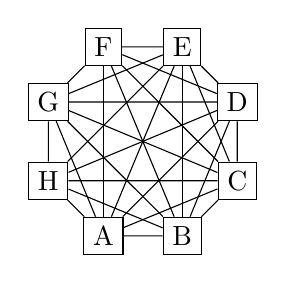
\begin{tikzpicture}
      \node[draw] (a) at (0,.3) {A};
      \node[draw] (b) at (1,.3) {B};
      \node[draw] (c) at (1.7,1) {C};
      \node[draw] (d) at (1.7,2) {D};
      \node[draw] (e) at (1,2.7) {E};
      \node[draw] (f) at (0,2.7) {F};
      \node[draw] (g) at (-.7,2) {G};
      \node[draw] (h) at (-.7,1) {H};
      \draw (a) -- (b) -- (c) -- (d) -- (e) -- (f) -- (g) -- (h) -- (a);
      \draw (a) -- (c) -- (h) -- (d) -- (g) -- (e);
      \draw (b) -- (h);
      \draw (b) -- (f);
      \draw (b) -- (d);
      \draw (b) -- (g);
      \draw (b) -- (e);
      \draw (h) -- (e);
      \draw (d) -- (f);
      \draw (g) -- (c);
      \draw (a) -- (d);
      \draw (a) -- (e);
      \draw (a) -- (f);
      \draw (a) -- (g);
      \draw (e) -- (c);
      \draw (c) -- (f);
    \end{tikzpicture}
\end{document}
%%% Local Variables: 
%%% mode: latex
%%% TeX-master: t
%%% End: 
 & \documentclass{standalone}
\usepackage{tikz}
\begin{document}
    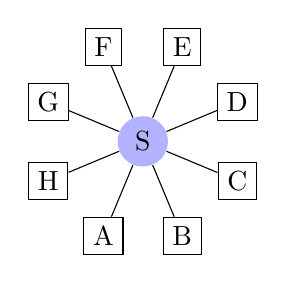
\begin{tikzpicture}
      \node[draw] (a) at (0,.3) {A};
      \node[draw] (b) at (1,.3) {B};
      \node[draw] (c) at (1.7,1) {C};
      \node[draw] (d) at (1.7,2) {D};
      \node[draw] (e) at (1,2.7) {E};
      \node[draw] (f) at (0,2.7) {F};
      \node[draw] (g) at (-.7,2) {G};
      \node[draw] (h) at (-.7,1) {H};
      \node[circle,fill=blue!30] (m) at (.5,1.5) {S};
      \draw (m) -- (a);
      \draw (m) -- (b);
      \draw (m) -- (c);
      \draw (m) -- (d);
      \draw (m) -- (e);
      \draw (m) -- (f);
      \draw (m) -- (g);
      \draw (m) -- (h);
    \end{tikzpicture}
\end{document}
%%% Local Variables: 
%%% mode: latex
%%% TeX-master: t
%%% End: 
 & \documentclass{standalone}
\usepackage{tikz}
\begin{document}
    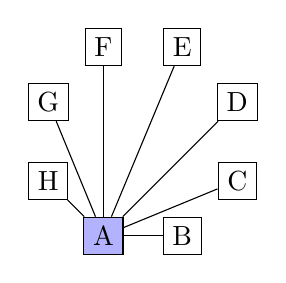
\begin{tikzpicture}
      \node[draw,fill=blue!30] (a) at (0,.3) {A};
      \node[draw] (b) at (1,.3) {B};
      \node[draw] (c) at (1.7,1) {C};
      \node[draw] (d) at (1.7,2) {D};
      \node[draw] (e) at (1,2.7) {E};
      \node[draw] (f) at (0,2.7) {F};
      \node[draw] (g) at (-.7,2) {G};
      \node[draw] (h) at (-.7,1) {H};
      \draw (a) -- (b);
      \draw (a) -- (c);
      \draw (a) -- (d);
      \draw (a) -- (e);
      \draw (a) -- (f);
      \draw (a) -- (g);
      \draw (a) -- (h);
    \end{tikzpicture}
\end{document}
%%% Local Variables: 
%%% mode: latex
%%% TeX-master: t
%%% End: 
\\\hline
    $n^2/2$  translations & $2n$ translations & $2n-2$ translations \\
    symmetric & symmetric & asymmetric\\\hline
  \end{tabular}
  \caption{Approaches for Safe Distributed Computation/Storage/UIs}\label{fig:interop}
\end{figure}
The first does not scale to a project with about a dozen systems, for the third there is
no obvious contender in the \ODK ecosystem. Fortunately, we already have a ``standard'' for
expressing the meaning of COMs -- \defemph{mathematical vernacular}: the language of
mathematical communication, and in fact all the COMs supported the \ODK VRE are documented
in mathematical vernacular in journal articles, manuals, etc.

The obvious problem is that mathematical vernacular is too 
\begin{inparaenum}[\em i\rm)]
\item \emph{ambiguous}: we need a human to understand structure, words, and symbols
\item \emph{redundant}: every paper introduces slightly different notions. 
\end{inparaenum}
Therefore we adopt an approach, where we partially formalize (\defemph{flexiformalize})
mathematical vernacular to obtain a flexiformal ontology of mathematics that can serve as
an open communication vocabulary. We call the approach the \defemph{Math-in-the-Middle}
(MitM) Strategy for integration and the ontology the MitM ontology\ednote{MK: I do not
  like this yet!}. 
\begin{wrapfigure}r{4cm}\vspace*{-1.5em}
  \documentclass{standalone}
\usepackage[mh]{mikoslides}
% this file defines root path local repository
\defpath{MathHub}{/Users/kohlhase/localmh/MathHub}
\mhcurrentrepos{MiKoMH/talks}
\libinput{WApersons}
% we also set the base URI for the LaTeXML transformation
\baseURI[\MathHub{}]{https://mathhub.info/MiKoMH/talks}

\usetikzlibrary{backgrounds,shapes,fit,shadows}
%\libinput{preamble}
\begin{document}
    \begin{tikzpicture}[scale=1.3]
      \tikzstyle{withshadow}=[draw,drop shadow={opacity=.5},fill=white]
      \tikzstyle{system}=[draw]
      \tikzstyle{standard}=[circle,fill=blue!30]
      \tikzstyle{interface}=[circle,fill=purple!30,inner sep = 1pt,]
      \node[system] (a) at (0,.3) {A};
      \node[system] (b) at (1,.3) {B};
      \node[system] (c) at (1.7,1) {C};
      \node[system] (d) at (1.7,2) {D};
      \node[system] (e) at (1,2.7) {E};
      \node[system] (f) at (0,2.7) {F};
      \node[system] (g) at (-.7,2) {G};
      \node[system] (h) at (-.7,1) {H};
      \node[standard] (m) at (.5,1.5) {S};
      \node[interface] (ia) at (0.2,.9) {a};
      \node[interface] (ib) at (.8,.9) {b};
      \node[interface] (ic) at (1.1,1.2) {c};
      \node[interface] (id) at (1.1,1.75) {d};
      \node[interface] (ie) at (.8,2.1) {e};
      \node[interface] (if) at (0.2,2.1) {f};
      \node[interface] (ig) at (-.1,1.75) {g};
      \node[interface] (ih) at (-.1,1.2) {h};
      \draw (m) -- (ia) -- (a);
      \draw (m) -- (ib) -- (b);
      \draw (m) -- (ic) -- (c);
      \draw (m) -- (id) -- (d);
      \draw (m) -- (ie) -- (e);
      \draw (m) -- (if) -- (f);
      \draw (m) -- (ig) -- (g);
      \draw (m) -- (ih) -- (h);
      \begin{pgfonlayer}{background}
        \node[draw,cloud,fit=(ia) (ib) (ic) (id) (ie) (if) (ig) (ih),
                   inner sep=-7pt,withshadow] (st) {};
        \node[fit=(d) (id),ellipse,inner sep=-1pt,rotate=20,draw,dashed,red] (sys) {};
      \end{pgfonlayer}
      \end{tikzpicture}
\end{document}
%%% Local Variables: 
%%% mode: latex
%%% TeX-master: t
%%% End: 
\vspace*{-.5em}
  \caption{Interface theories}\label{fig:interface-theories}\vspace*{-1em}
\end{wrapfigure}
Before we go into any detail about how this ontology looks and how it induces a uniform
meaning space, we have to address another problem: the descriptions in the MitM ontology
must at the same time be system-near, to make interfacing easy for systems, and serve as
an interoperability standard -- i.e. be general and stable. If we have an ontology system
that allows modular/structured ontologies, we can solve this apparent dilemma by
introducing \defemph{interface theories}~\cite{KohRabSac:fvip11}, i.e. ontology modules
(the light purple circles in Figure~\ref{fig:interface-theories}) that are at the same
time system-specific in their description of COMs -- near the actual representation of the
system and part of the greater MitM ontology (depicted by the cloud in
Figure~\ref{fig:interface-theories}) as they are connected to the core MitM ontology (the
blue circle) by views we call \defemph{interviews} (see below). The MitM approach
stipulates that interface theories and interviews maintained and released together with
the respective systems, whereas the core MitM ontology represents the mathematical scope
of the VRE and is maintained with it. In fact in many ways, the core MitM ontology is the
conceptual essence of the mathematical VRE.

\subsection{Realizing and Utilizing a MitM Ontology}

\begin{wrapfigure}r{6cm}\centering\vspace*{-2em}
  \documentclass{standalone}
\usepackage{tikz}
\usetikzlibrary{mmt}
\def\cn#1{\ensuremath{\mathsf{#1}}}
\begin{document}
\providecommand\myyscale{1}
\providecommand\myxscale{.9}
\begin{tikzpicture}[xscale=\myxscale,yscale=\myyscale]
% \draw[view] (-4,2.4) --node[above] {translation} +(2,0);
% \draw[struct] (-4,1.7) --node[above] {import} +(2,0);
% \draw[meta] (-4,1) --node[above] {meta-theory} +(2,0);
\node[thy] (lf) at (0,2.5)  {$\cn{LF}$};
\node[thy] (lfx) at (1.8,2.5)  {$\cn{LF+X}$};
\node[thy] (fol) at (-1,1.5)   {$\cn{FOL}$};
\node[thy] (hol) at (.9,1.5) {$\cn{HOL}$};
\node[thy] (mon) at (-2.5,0) {$\cn{Monoid}$};
\node[thy] (gp) at (-.5,0) {$\cn{CGroup}$};
\node[thy] (rg) at (2,0)  {$\cn{Ring}$};
\node[thy] (zfc) at (-2.8,1.5) {$\cn{ZFC}$};

\draw[meta](lf) -- (fol);
\draw[meta](lf) -- (hol);
\draw[meta](fol) -- (mon);
\draw[meta](fol) -- (gp);
\draw[meta](hol) -- (rg);
\draw[include](lf) -- (lfx);
\draw[view](fol) -- node[above] {\footnotesize$\cn{f2h}$} (hol);
\draw[struct](gp) to[bend right=10] node[above] {\footnotesize$\cn{add}$} (rg);
\draw[struct](mon) to[out=20,in=160] node[above] {\footnotesize$\cn{mult}$} (rg);
\draw[include](mon) -- (gp);
\draw[view] (fol) -- node[above]{\footnotesize$\cn{folsem}$} (zfc);
\draw[view] (mon) -- node[right,near end]{\footnotesize$\cn{mod}$} (zfc);
\end{tikzpicture}
\end{document}
%%% Local Variables:
%%% mode: latex
%%% TeX-master: t
%%% End:
\vspace*{-.5em}
  \caption{OMDoc/MMT Theory Graphs}\label{fig:mmt}\vspace*{-1em}
\end{wrapfigure}
We use the OMDoc/MMT format~\cite{Kohlhase:OMDoc1.2,MMTSVN:on} to represent the MitM
ontology. OMDoc/MMT is an ontology format specialized to representing mathematical
knowledge modularly in a theory graph: \defemph{theories} are collections of declarations
of concepts, objects, and their properties that are connected by truth-preserving mappings
called \defemph{theory morphisms}. The latter come in two forms: \defemph{inclusions} and
\defemph{structures} that essentially correspond to object-oriented inheritance, and
\defemph{view} that connect pre-existing theories -- in these all axioms of the source
theory have be to proven in the target theory. See ~\cite{RabKoh:WSMSML13} for a full
account. 

Figure~\ref{fig:mmt} shows an example theory graph. It has three layers:
\begin{compactenum}[\em i\rm)]
\item the \defemph{domain level}, which specifies mathematical domains as theories; here
  parts of elementary algebra. The hooked arrows are inclusions for inheritance the
  regular arrows are named structures that induce the additive and multiplicative
  structures of a ring.
\item the \defemph{logic level} represents the languages we use for talking about the
  properties of the objects at the domain level -- again as theories: the meta-theories of
  the domain-level ones -- the dotted arrows signify the meta-relation. At this level, we
  also have inclusions and views (the squiggly arrows) which correspond to logic
  translations (\cn{f2h}) and interpretations into \defemph{foundational theories} like
  set theory (here \cn{ZFC}). Incidentally models can be represented as views into
  foundations.
\item The top layer contains theories that act as metalogics, e.g. the Logical Framework
  \cn{LF} and extensions which can be used to specify logics and their translations.
\end{compactenum}
The theory graph structure is very well-suited to represent heterogeneous collections of
mathematical knowledge, because views at the domain level can be used to connect differing
but equivalent conceptualizations and views at the logic level can be used to bridge the
different foundations of the various systems. The top level is only indirectly used in in
the MitM framework: it induces the joint meaning space via the meta-relation.

\begin{figure}[ht]\centering
  \documentclass{standalone}
\usepackage[mh]{mikoslides}
% this file defines root path local repository
\defpath{MathHub}{/Users/kohlhase/localmh/MathHub}
\mhcurrentrepos{MiKoMH/talks}
\libinput{WApersons}
% we also set the base URI for the LaTeXML transformation
\baseURI[\MathHub{}]{https://mathhub.info/MiKoMH/talks}

\usetikzlibrary{backgrounds,shapes,fit,shadows,mmt}
\begin{document}
\begin{tikzpicture}[xscale=2.6,yscale=.9]
  \tikzstyle{withshadow}=[draw,drop shadow={opacity=.5},fill=white]
   \tikzstyle{database} = [cylinder,cylinder uses custom fill,
      cylinder body fill=yellow!50,cylinder end fill=yellow!50,
      shape border rotate=90,
      aspect=0.25,draw]
   \tikzstyle{human} = [red,dashed,thick]
   \tikzstyle{machine} = [green,dashed,thick]

\node[thy]  (mf) at (.2,5.3) {MathF};
\node[thy,dashed]  (compf) at (0,6) {CompF};
\node[thy,dashed]  (pf) at (-.9,5.5) {PyF};
\node[thy,dashed]  (cf) at (1,5.5) {C\textsuperscript{++}F};
\node[thy,dashed]  (sf) at (-0.9,4.6) {SAGE};
\node[thy,dashed]  (gf) at (1,4.6) {GAP};

\draw[include] (compf) -- (pf);
\draw[includeleft] (compf) -- (cf);
\draw[include] (pf) -- (sf);
\draw[includeleft] (cf) -- (gf);

\node[thy] (kec) at (0,3) {EC};
\node[thy,minimum height=.4cm] (kl) at (0,4) {\ldots};

\node[thy] (sec) at (-1,2) {SEC};
\node[thy,minimum height=.4cm] (sl) at (-1,3) {\ldots};

\node[thy] (gec) at (1,2) {GEC};
\node[thy,minimum height=.4cm] (gl) at (1,3) {\ldots};

\node[thy] (lec) at (-.3,1.2) {LEC};
\node[thy,minimum height=.4cm] (ll) at (.3,1.2) {\ldots};

\node (sc) at (-2,4) {SAGE};
\node[draw] (salg) at (-2,3.35) {Algo};
\node[database,dashed] (sdb) at (-2,2.4) {DB?};
\node[draw] (skr) at (-2,1.7) {KR};
\node[draw,machine] (sac) at (-2,1) {AbsClass};

\node (gc) at (2,4) {GAP};
\node[draw] (galg) at (2,3.35) {Algo};
\node[database,dashed] (gdb) at (2,2.4) {DB?};
\node[draw] (gkr) at (2,1.7) {KR};
\node[draw,machine] (gac) at (2,1) {AbsClass};

\node (lmfdb) at (0,0) {LMFDB};
\node[database] (ldb) at (1,-.4) {Mongo};
\node[draw] (knowls) at (-1,-.4) {Knowls};
\node[draw,machine] (lac) at (0,-.5) {AbsClass};

  \begin{pgfonlayer}{background}
    \node[draw,cloud,fit=(sec) (sl),aspect=.4,inner sep=-3pt,withshadow,purple!30] (st) {};
    \node[draw,cloud,fit=(gec) (gl),aspect=.4,inner sep=-4pt,withshadow,purple!30] (gt) {};
    \node[draw,cloud,fit=(kec) (kl),aspect=.4,inner sep=0pt,withshadow,blue!30] (kt) {};
    \node[draw,cloud,fit=(lec) (ll),aspect=2.5,inner sep=-7pt,withshadow,purple!30] (lt) {};
  \end{pgfonlayer}

\begin{pgfonlayer}{background}
  \node[draw,withshadow,fit=(sc) (skr) (sac) (sdb),inner sep=1pt] {};
  \node[draw,withshadow,fit=(gc) (gkr) (gac) (gdb),inner sep=1pt] {};
  \node[draw,withshadow,fit=(lmfdb) (lac) (ldb) (knowls),inner sep=1pt] {};
\end{pgfonlayer}

\draw[view] (kec) -- (sec);
\draw[view] (kec) -- (gec);
\draw[view] (kec) -- (lec);
\draw[include] (kec) -- (kl);
\draw[include] (gec) -- (gl);
\draw[include] (sec) -- (sl);
\draw[include] (lec) -- (ll);
\draw[view] (kl) -- (sl);
\draw[view] (kl) -- (gl);
\draw[view] (kl) to[bend left=5] (ll);

\draw[meta] (mf)  to [bend right=10] (st);
\draw[meta] (sf) -- (st);
\draw[meta] (mf)  to [bend left=10] (gt);
\draw[meta] (gf) -- (gt);
\draw[meta] (mf) -- (kt);
\draw[meta] (compf) to[bend right=15] (kt);

\draw[human,->] (skr) -- node[above]{\scriptsize edit} (st);
\draw[human,->] (gkr) -- node[above]{\scriptsize edit} (gt);
\draw[human,->] (knowls) -- node[left,near end]{\scriptsize edit} (lt);

\draw[machine,->] (gt) to[bend right=30] node[below,near start]{\scriptsize generate} (gac);
\draw[machine,->] (st) to[bend left=30] node[below,near start]{\scriptsize generate} (sac);
\draw[human,->] (st) to[bend left=20] node[below]{\scriptsize refactor} (kt);
\draw[human,->] (gt) to[bend right=20] node[below]{\scriptsize refactor} (kt);
\draw[human,->] (lt) -- node[right]{\scriptsize refactor} (kt);
\end{tikzpicture}
\end{document}
%%% Local Variables: 
%%% mode: latex
%%% TeX-master: t
%%% End: 

  \caption{The MitM Paradigm in Details}\label{fig:mitm}
\end{figure}
If we apply OMDoc/MMT to the MitM architecture, we arrive at the situation in
Figure~\ref{fig:mitm}, where we drill into the MitM information architecture from
Figure~\ref{fig:interface-theories}, but restrict to three systems from the \ODK
project. In the middle we see the core MitM ontology (the blue cloud) as an OMDoc/MMT
theory graph connected to the interface theories (the purple clouds) via MitM
interviews. Conceptually, the systems in \ODK consist of three main components:
\begin{inparaenum}[\em i\rm)]
\item a \emph{knowledge representation subsystem} that provides data structures for the COMs and
  their properties.
\item a \emph{database component} that provides mass storage for objects, and 
\item a \emph{library of algorithms} that operate on these.
\end{inparaenum}
To connect a system to an MitM-based VRE, the KR subsystem is either refactored so that it
can generate interface theories, or a schema-like description of the underlying data
structures is created manually from which abstract data structures for the system can be
generated automatically -- in this version the interface theories act as an Interface
Description Language.

In this situation there are two ways to arrive at a greater MitM ontology: the \ODK
project aims to explore both: either
\begin{inparaenum}[\em i\rm)] 
\item standardizing a core MitM by refactoring the various interface theories where they
  overlap, or
\item flexiformalizing the available literature for a core MitM ontology.
\end{inparaenum}
For \emph{i}), the MitM interviews emerge as refinements that add system-specific detail
to the general mathematical concepts\footnote{We use the word ``interface theory'' with a
  slightly different intention when compared to the original use
  in~\cite{KohRabSac:fvip11}: There the core MitM ontology would be an interface between
  the more specific implementations in the systems, whereas here we use the ``interface
  theories'' as interfaces between systems and the core MitM ontology. Technically the
  same issues apply.} For \emph{ii}), we have to give the interviews directly. 

To see that this architecture indeed gives us a uniform meaning space, we observe that the
core MitM ontology uses a mathematical foundation (presumably some form of set theory),
whereas the interface theories also use system-specific foundations that describe aspects
of the computational primitives of the respective systems. We have good formalizations of
the mathematical foundations already; first steps towards a computational ones have been
taken in~\cite{KohManRab:aumftg13}

%%% Local Variables:
%%% mode: latex
%%% TeX-master: "paper"
%%% End:

%  LocalWords:  pn visualization lstinline ec lstinline Weierstrass ednote interop hline
%  LocalWords:  centering tikz fullgraph tikz mstargraph tikz stargraph defemph emph mmt
%  LocalWords:  inparaenum flexiformalize flexiformal wrapfigure vspace mistargraph cn
%  LocalWords:  KohRabSac fvip11 Realizing Utilizing metalogics specialized RabKoh mitm
%  LocalWords:  compactenum conceptualizations kf-paradigm standardizing flexiformalizing
%  LocalWords:  formalizations KohManRab aumftg13
